%%%%%%%%%%%%%%%%%%%%%%%%%%%%%%%%%%%%%%%%%%%%%%%%%%%%%%%%%%%%%%%
%
% Welcome to Overleaf --- just edit your LaTeX on the left,
% and we'll compile it for you on the right. If you open the
% 'Share' menu, you can invite other users to edit at the same
% time. See www.overleaf.com/learn for more info. Enjoy!
%
%%%%%%%%%%%%%%%%%%%%%%%%%%%%%%%%%%%%%%%%%%%%%%%%%%%%%%%%%%%%%%%
\documentclass[landscape]{article}

\usepackage[legalpaper,bindingoffset=0.2in,%
            left=1cm,right=1cm,top=1in,bottom=1in,%
            footskip=.25in]{geometry}
            
\usepackage{tikz}
\usepackage{verbatim}

\begin{comment}
:Title: Neural network
:Tags: Foreach

The ``\foreach`` command is very useful for quickly creating structured graphics
like this neural network diagram.

\end{comment}

\begin{document}
\pagestyle{empty}

\def\layersep{3.5cm}

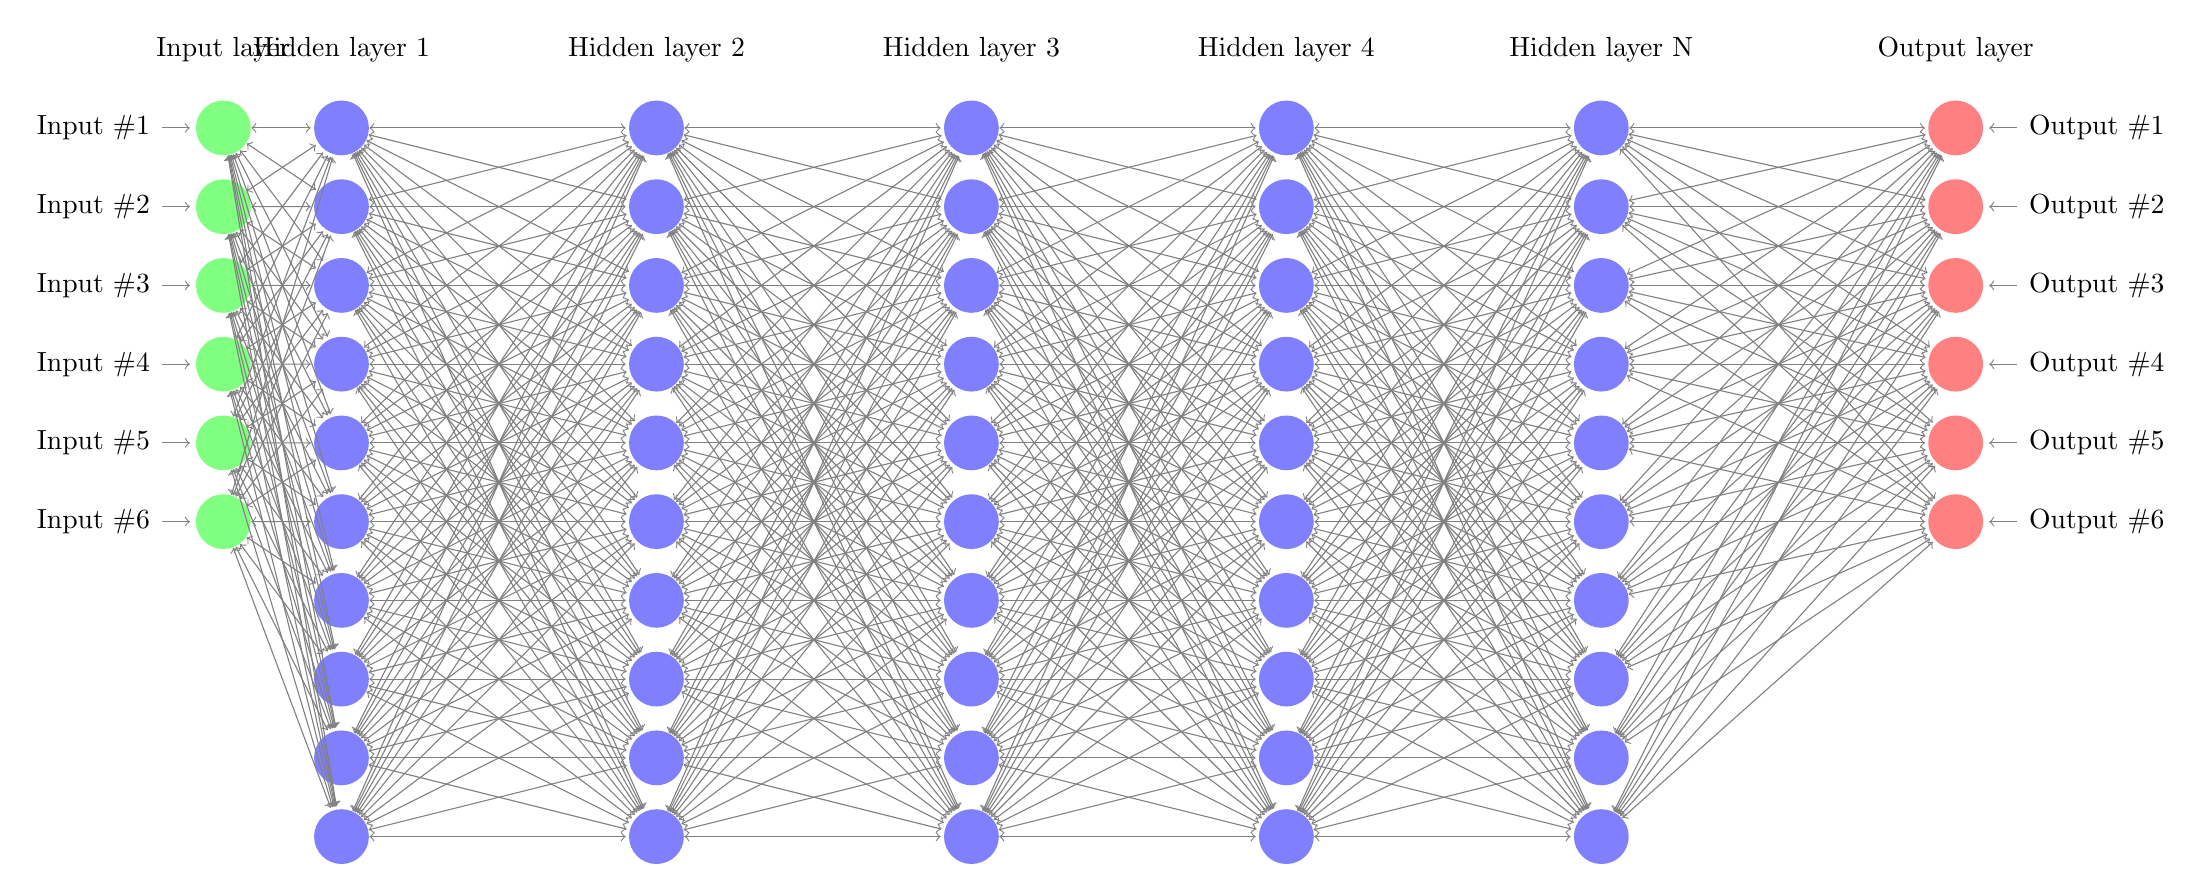
\begin{tikzpicture}[shorten >=1pt,<->,draw=black!50, node distance=\layersep]
    \tikzstyle{every pin edge}=[<-,shorten <=2pt]
    \tikzstyle{neuron}=[circle,fill=black!25,minimum size=5pt,inner sep=7pt]
    \tikzstyle{input neuron}=[neuron, fill=green!50];
    \tikzstyle{output neuron}=[neuron, fill=red!50];
    \tikzstyle{hidden neuron}=[neuron, fill=blue!50];
    \tikzstyle{annot} = [text width=10em, text centered]

    % Draw the input layer nodes
    \foreach \name / \y in {1,...,6}
    % This is the same as writing \foreach \name / \y in {1/1,2/2,3/3,4/4}
        \node[input neuron, pin=left:Input \#\y] (I-\name) at (0,-\y) {};

    % Draw the hidden layer nodes
    \foreach \name / \y in {1,...,10}
        \path[xshift=.5cm]
            node[hidden neuron] (H1-\name) at (\layersep,-\y cm) {};

    % Draw the hidden layer 2 nodes
    \foreach \name / \y in {1,...,10}
        \path[xshift=4.5cm]
            node[hidden neuron] (H2-\name) at (\layersep,-\y cm) {};

    % Draw the hidden layer 3 nodes
    \foreach \name / \y in {1,...,10}
        \path[xshift=8.5cm]
            node[hidden neuron] (H3-\name) at (\layersep,-\y cm) {};

    % Draw the hidden layer 4 nodes
    \foreach \name / \y in {1,...,10}
        \path[xshift=12.5cm]
            node[hidden neuron] (H4-\name) at (\layersep,-\y cm) {};

    % Draw the hidden layer N nodes
    \foreach \name / \y in {1,...,10}
        \path[xshift=16.5cm]
            node[hidden neuron] (HN-\name) at (\layersep,-\y cm) {};

    % Draw the output layer nodes
    \foreach \name / \y in {1,...,6}
        \path[xshift=21cm]
            node[output neuron, pin=right:Output \#\y] (O-\name) at (\layersep,-\y cm) {};

    % Draw the output layer node
    %\node[output neuron,pin={[pin edge={->}]right:Output}, right of=H-3] (O) {};

    % Connect every node in the input layer with every node in the
    % hidden layer 1
    \foreach \source in {1,...,6}
        \foreach \dest in {1,...,10}
            \path (I-\source) edge (H1-\dest);

    % hidden layer 2
    \foreach \source in {1,...,10}
        \foreach \dest in {1,...,10}
            \path (H1-\source) edge (H2-\dest);

    % hidden layer 3
    \foreach \source in {1,...,10}
        \foreach \dest in {1,...,10}
            \path (H2-\source) edge (H3-\dest);

    % hidden layer 4
    \foreach \source in {1,...,10}
        \foreach \dest in {1,...,10}
            \path (H3-\source) edge (H4-\dest);

    % hidden layer N
    \foreach \source in {1,...,10}
        \foreach \dest in {1,...,10}
            \path (H4-\source) edge (HN-\dest);

    % Connect every node in the hidden layer with the output layer
    \foreach \source in {1,...,10}
        \foreach \dest in {1,...,6}
            \path (HN-\source) edge (O-\dest);

    % Annotate the layers
    \node[annot,above of=H1-1, node distance=1cm] (hl) {Hidden layer 1};
    \node[annot,above of=H2-1, node distance=1cm] (hl) {Hidden layer 2};
    \node[annot,above of=H3-1, node distance=1cm] (hl) {Hidden layer 3};
    \node[annot,above of=H4-1, node distance=1cm] (hl) {Hidden layer 4};
    \node[annot,above of=HN-1, node distance=1cm] (hl) {Hidden layer N};
    \node[annot,above of=I-1, node distance=1cm] {Input layer};
    \node[annot,above of=O-1, node distance=1cm] {Output layer};
\end{tikzpicture}
% End of code
\end{document}
